\documentclass[review]{elsarticle}

\usepackage{lineno,hyperref}
\usepackage{color}
\usepackage[showframe=false]{geometry}
\usepackage{amsmath,amsfonts,amssymb}
\usepackage{float}
\usepackage{graphicx}
\usepackage{epstopdf}
\usepackage{subfigure}
\usepackage{mathtools}
\usepackage[table]{xcolor}
\usepackage{changepage}
%%%%%%%%%%%%%%%%%%%%%%%%
% for revision
\usepackage{ulem}
\modulolinenumbers[5]

\journal{Annals of Nuclear Engineering}

%%%%%%%%%%%%%%%%%%%%%%%
%% Elsevier bibliography styles
%%%%%%%%%%%%%%%%%%%%%%%
%% To change the style, put a % in front of the second line of the current style and
%% remove the % from the second line of the style you would like to use.
%%%%%%%%%%%%%%%%%%%%%%%

%% Numbered
%\bibliographystyle{model1-num-names}

%% Numbered without titles
%\bibliographystyle{model1a-num-names}

%% Harvard
%\bibliographystyle{model2-names.bst}\biboptions{authoryear}

%% Vancouver numbered
%\usepackage{numcompress}\bibliographystyle{model3-num-names}

%% Vancouver name/year
%\usepackage{numcompress}\bibliographystyle{model4-names}\biboptions{authoryear}

%% APA style
%\bibliographystyle{model5-names}\biboptions{authoryear}

%% AMA style
%\usepackage{numcompress}\bibliographystyle{model6-num-names}

%% `Elsevier LaTeX' style
\bibliographystyle{elsarticle-num}
%%%%%%%%%%%%%%%%%%%%%%%
\newcommand{\zh}{ZrH$_x$}
\newcommand{\e}[1]{\ensuremath{\times10^{#1}}}
\newcommand{\tcr}[1]{\textcolor{blue}{\textbf{#1}}}
\newcommand{\TAMU}{Texas A\&M University}
\newcommand{\ddxcs}{\sigma(E'\to E,~\mu)}
\newcommand{\law}{S(\alpha,\beta)}
\newcommand{\dxcs}{\sigma_l(E'\to E)}
\newcommand{\ekt}{\frac{E}{kT}}
\newcommand{\epkt}{\frac{E'}{kT}}
\newcommand{\erf}{\mathrm{erf}}
\newcommand{\fgp}{F_\mathrm{g'}}
\newcommand{\sgg}{\sigma_{l,\mathrm{g'}\to \mathrm{g}}}
\newcommand{\eg}{E_\mathrm{g}}
\newcommand{\egp}{E_\mathrm{g'}}
\newcommand{\ego}{E_\mathrm{g+1}}
\newcommand{\egpo}{E_\mathrm{g'+1}}
\newcommand{\psig}{\psi_\mathrm{g}(\vec{r},\mathbf{\Omega})}
%\newcommand{\and}{\qquad\mathrm{and}\qquad}

%\newcommand{\sb1}{\hat{\sigma}_\mathrm{b}}
\begin{document}

\begin{frontmatter}

\title{Semi-analytic Benchmark for Multi-group Free-gas Legendre Moments and the Application of Gauss quadrature in Generating Thermal Scattering Legendre Moments}
%\tnotetext[mytitlenote]{Fully documented templates are available in the elsarticle package on \href{http://www.ctan.org/tex-archive/macros/latex/contrib/elsarticle}{CTAN}.}

%% Group authors per affiliation:
\author[mymainaddress]{Weixiong Zheng}
\ead{zwxne2010@tamu.edu}
%% or include affiliations in footnotes:
%\author[mymainaddress,mysecondaryaddress]{Elsevier Inc}
%\ead[url]{www.elsevier.com}

\author[mymainaddress]{Ryan G. McClarren\corref{mycorrespondingauthor}}
\cortext[mycorrespondingauthor]{Corresponding author}
\ead{rgm@tamu.edu}

\address[mymainaddress]{Nuclear Engineering, \TAMU,~College Station, TX 77843-3133}

\begin{abstract}
As high-fidelity simulations become routine and computational modelers begin to ask questions about uncertainty in calculations, the understanding of uncertainties in nuclear data, including multigroup cross-sections to high scattering orders, is also becoming important. In this paper we look at how a widely-used data processing code, NJOY, processes thermal cross-section data.  Using an alternative integration scheme, Gauss quadrature, for angular integration to generate thermal scattering cross sections from the thermal scattering laws for graphite and \zh,~we observed discrepancies between these results and NJOY's results using equal-probable cosines on high order Legendre moments. In order to find a reliable comparison between the methods in NJOY and alternatives, we derived novel analytical expressions for high order Legendre moments of the free gas scattering model. Such expressions are analytically tractable but complicated. Using these expressions we construct a semi-analytic benchmark for multigroup Legendre moments. By comparing the results among the benchmark, Gauss quadrature and NJOY, we found that Gauss quadrature can preserve comparable accuracy as NJOY for lower order Legendre moments for free gas scattering and outperforms NJOY in generating high order moments. Our findings indicate that for high-scattering moments, multigroup data could be an source of uncertainty in thermal reactor calculations.
\end{abstract}

\begin{keyword}
Benchmark Solutions\sep Legendre order\sep Free gas \sep Gauss quadrature\sep Equal probable cosine
\end{keyword}

\end{frontmatter}

\linenumbers

\section{Introduction}
\subsection{Background}
In nuclear reactors, neutron behavior is described by neutron transport equation. In particular, the steady state neutron transport equation with multi-group approximation in reactor analysis can be generalized as\cite{handbooktransportequation}:
\begin{align}
\mathbf{\Omega}\cdot\nabla\psi_\mathrm{g}(\vec{r},\mathbf{\Omega})+\Sigma_\mathrm{t,g}\psig=\sum\limits_{\mathrm{g'}=1}^{G}\int\limits_{4\pi}d\Omega'\ \Sigma_\mathrm{s,g'\to g}(\vec{r},\mathbf{\Omega'\cdot\Omega})\psi_\mathrm{g'}(\vec{r},\mathbf{\Omega'})\\
+\frac{S_\mathrm{f,g}(\vec{r})}{4\pi}+\frac{Q_\mathrm{g}(\vec{r})}{4\pi},\mathrm{g}=1,\cdots,G\nonumber
\end{align} 
where the $\psi_\mathrm{g}$\ is the average angular flux in $\mathrm{g^{th}}$\ energy group; $\Sigma_\mathrm{t,g}$\ is the macroscopic total cross section for group g; $\Sigma_\mathrm{s,g'\to g}$\ is the macroscopic scattering cross section from group g' to g; $S_\mathrm{f,g}$\ and $Q_\mathrm{g}$\ represents group averaged fission source and distributed source for group g.

Specifically, the scattering cross section can be defined as:
\begin{equation}
\Sigma_\mathrm{s,g'\to g}(\vec{r},\mathbf{\Omega'\cdot\Omega})=\sum\limits_{l=0}^{L}\frac{2l+1}{4\pi}\sum\limits_{\mathrm{i=1}}^{\mathrm{I}}N_\mathrm{i}(\vec{r})\sigma_{l\mathrm{,g'\to g}}^{\mathrm{(i)}}(\vec{r})P_l(\mathbf{\Omega'\cdot\Omega}),
\end{equation}
where $N_\mathrm{i}$ is the atom density of i$^{\mathrm{th}}$\ nuclide and $\sigma_{l,\mathrm{,g'\to g}}$\ is the l$^{\mathrm{th}}$\ moment of microscopic scattering cross section from group g' to g for i$^{\mathrm{th}}$ type of nuclide. The scattering events become part of the neutron source that in order to obtain plausible solution of the transport equation, accurate estimation of the scattering Legendre moments is needed.


At thermal energies, scattering in some mediums is associated with molecular structure and therefore becomes complex\cite{IKE,Macf,thesis}. Among the subtypes of reactions under the category of thermal neutron scattering\footnote{There are three types of thermal neutron scattering, i.e.,\ incoherent inelastic, incoherent elastic and coherent elastic scatterings. Interested readers may refer to Refs.\ \cite{IKE,njoy2012}\ for more detailes}, we restrict the analysis in this paper to thermal incoherent inelastic as it heavily affects the upscattering and accurate calculation of Legendre moments of this type of scattering is difficult\cite{glasstone}. However, uncertainties in thermal scattering cross sections can propagate through the reactor simulation and therefore are sensitively connected to accuracy of criticality calculations\cite{emulation,Badea,IKE,thesis,weixiong,physor},\ it is then important to develop effective algorithms to carry out the data processing and also investigate the validity of the algorithms in existing codes,\,e.g.,\,NJOY\cite{NJOY},\ on data generation.

%\textcolor{blue}{Accurate evaluation of neutron scattering Legendre moment is highly demanded in order to characterize the scattering in reactor transport simulations. Some works have been done on effective evaluatation of scattering Legendre moments\cite{transfercrosssection}.\,Since uncertainties in the cross section can be propogated through transport calculations and therefore sensitively connected with accuracy of criticality calculations\cite{emulation,Badea}, it is important to develop effective algorithms carrying out the scattering data processing. Also, investigation on validity of the algorithms in existing codes is significant to gain insight into uncertainty of the generated scattering data. Specifically, at thermal energies the scattering becomes associated with material molecular structrure and therefore more complex\cite{weixiong,physor,thesis}. Specifically, in this work, we restrict ourselves to thermal \textcolor{red}{incoherent inelastic} scattering cross section calculations due to its impact on upscattering. This fact leads to further challenge for correctly estimating the scattering moments.}

NJOY is a powerful code at the state of art in nuclear cross section processing\footnote{In this paper, NJOY 99.0 was used.}. For thermal scattering reactions, different modules, e.g.~LEAPR, THERMR and GROUPR, perform necessary tasks from generating continuous-energy (CE) scattering cross sections from scattering kernels through group collapse to computing multigroup Legendre moments of scattering\cite{NJOY}. When synthesizing multiple orders of Legendre moments, NJOY invokes a method that adaptively seeks equal probable cosines (EPC) and scattering angular probability density function for each embedded incident energy point and calculates the zeroth Legendre moment\cite{NJOY,Macf}. Under proper assumptions, CE Legendre moments up to any user designated order can be  approximated. We refer to this method as the ``EPC" method. This algorithm is computationally efficient since the code does not directly calculate each non-zeroth order of Legendre moments through angular integration. The details will be introduced in the following sections.

Recently, we developed a code to generate multigroup constants for the thermal scattering of \zh~and graphite. Instead of the algorithm NJOY uses to generate Legendre moments, we used numerical integration with Gauss quadrature to achieve every order of the CE Legendre moments individually. 
An interesting observation is that though the multigroup moments from both codes agree with each other at low order, discrepancies occur to the high order moments, especially when the difference between incident energy and outgoing energy is large. Moreover, reducing energy intervals in group collapse does not improve the agreement between results from two methods. The difference between the Gauss quadrature and NJOY's results did not go away as the quadrature order is increased.

Synthesizing group constants for real materials is a complex process. To produce the thermal scattering group cross sections, one needs to have a functional form of the phonon spectrum. Typically this is written as $\law$,~which is a function of two variables $\alpha$,~the momentum transfer, and $\beta$,~the energy transfer, in the scattering event. The function $\law$~is known as the thermal scattering law and is connected to the temperature of the material $T$, and the phonon spectrum,
%\begin{equation}
%\law=F(f(\omega),T),
%\end{equation}
%where 
$f(\omega)$, where $\omega$~is the phonon energy. The variables $\alpha$~and $\beta$~are the momentum transfer and energy transfer, respectively:
\begin{equation}
\alpha\equiv\frac{E+E'-2\mu\sqrt{EE'}}{AkT}\qquad\mathrm{and}\qquad\beta\equiv\frac{E-E'}{kT},
\end{equation}
where $E'$~and $E$~are the incident and secondary neutron energies, $\mu$~is the cosine of scattering angle between incident and outgoing directions, i.e.,\,$\mu=\mathbf{\Omega'\cdot\Omega}$.\ $A$~represents the ratio of the scatterer (such as H in \zh)~mass to neutron mass. 

The double differential scattering cross section, $\ddxcs$,~is associated with the scattering law by:
\begin{equation}\label{ddx}
\ddxcs=\frac{\hat{\sigma}_\mathrm{b}}{2kT}\sqrt{\frac{E}{E'}}S(\alpha,~\beta),
\end{equation}
where $\hat{\sigma}_\mathrm{b}$~is the thermal neutron scattering characteristic cross section in bound systems \cite{neutronnews}. In order to test the efficacy of Gauss quadrature in calculating thermal scattering Legendre moments, we derive benchmark models using simple scattering kernels, such as the free gas model. The free gas model is advantageous since the scattering kernel is a delta function, making the scattering law analytic \cite{Macf,IKE}. Furthermore, with such an analytic scattering law, it is possible to derive the CE scattering cross section for any order analytically. Such analytic results could then be used as benchmarks for any methods for computing scattering cross sections.
\section{Formulations}
It is straightforward to derive differential scattering moments, $\dxcs$,~from Eq.~\eqref{ddx}:
\begin{equation}\label{dx}
\dxcs=\int\limits_{-1}^{1}d\mu\ P_l(\mu)\ddxcs,~l=0,1,\cdots,
\end{equation}
where $l$~is the order of the Legendre moments and $P_l(\mu)$~is the Legendre polynomial at point $\mu$.

There are numerous ways to implement the above integration. One could use different quadratures to directly accomplish the goal for each order individually. On the other hand, one could also use the aforementioned EPC method as follows.
\subsection{EPC method}
%It would be computationally expensive to implement Eq.~\eqref{dx}~if several orders of moments are needed in transport simulations. The EPC method avoids this drawback by skipping the direct calculation of all moments.
The EPC method was developed to calculate CE Legendre scattering moments effectively. 
The double differential scattering cross section can be expressed as a product of the zeroth moment and corresponding term $p(\mu|E')$:
\begin{equation}
\ddxcs=\sigma_0(E'\to E)p(\mu|E'),
\end{equation}
where $\sigma_0$~is the differential scattering cross section, which is also the zeroth order of the differential scattering moments, and $p(\mu|E')$~is the angular probability density function for thermal neutrons with incident energy of $E'$ which is normalized such that $\int\limits_{-1}^{1}d\mu\ p(\mu|E')=1$.

Denote $N$~as the number of angular bins, then if each bin is equally probable, we have:
\begin{equation}
\int\limits_{\mu_\mathrm{i}}^{\mu_\mathrm{i+1}}d\mu\,p(\mu|E')=\frac{1}{N},\qquad\mathrm{i}=1,2,\cdots,N,
\end{equation}
where $\mu_\mathrm{i}$~and $\mu_\mathrm{i+1}$~are the lower and upper bounds of the $\mathrm{i}^\mathrm{th}$~bin, respectively.

NJOY calculates $\sigma_0$\ and adaptively derive a cosine set $\{\hat{\mu}_\mathrm{i}\}_\mathrm{i=1}^N$ at each incident energy such that the average cosine can be preserved in the corresponding bin\cite{njoy2012}:
%\begin{equation}\label{epc}
%p(\hat{\mu}_\mathrm{i}|E')\left(\mu_\mathrm{i+1}-\mu_\mathrm{i}\right)=\int\limits_{\mu_\mathrm{i}}^{\mu_\mathrm{i+1}}d\mu\,p(\mu|E')=\frac{1}{N},\qquad\hat{\mu_{\mathrm{i}}}\in(\mu_\mathrm{i},\mu_\mathrm{i+1})
%\end{equation}
\begin{equation}\label{epc}
\hat{\mu}_\mathrm{i}=\frac{\displaystyle\int\limits_{\mu_\mathrm{i}}^{\mu_\mathrm{i+1}}d\mu\ \mu\sigma(E'\to E,\mu)}{\displaystyle\frac{1}{N}\int\limits_{-1}^{1}d\mu\ \sigma(E'\to E,\mu)}
\end{equation}
where $\hat{\mu_\mathrm{i}}$~is the equal probable cosine.

Use these cosines and assume:
\begin{equation}\label{e:apps}
\int\limits_{\mu_\mathrm{i}}^{\mu_\mathrm{i+1}}d\mu\ P_l(\mu)p(\mu|E')\sigma_0(E'\to E)\approx\int\limits_{\mu_\mathrm{i}}^{\mu_\mathrm{i+1}}d\mu\ P_l(\hat{\mu}_\mathrm{i})\sigma_0(E'\to E)p(\mu|E')=P_l(\hat{\mu}_\mathrm{i})\int\limits_{\mu_\mathrm{i}}^{\mu_\mathrm{i+1}}d\mu\ \sigma_0(E'\to E)p(\mu|E')
\end{equation} 
one can show:
\begin{align}
\dxcs&=\int\limits_{-1}^{1}d\mu\ P_l(\mu)p(\mu|E')\sigma_0(E'\to E)\nonumber\\
&=\sum\limits_{\mathrm{i=1}}^{N}\int\limits_{\mu_\mathrm{i}}^{\mu_\mathrm{i+1}}d\mu\ P_l(\mu)\sigma_0(E'\to E)p(\mu|E')\\
&\approx\sum\limits_{\mathrm{i=1}}^{N}P_l(\hat{\mu}_\mathrm{i})\int\limits_{\mu_\mathrm{i}}^{\mu_\mathrm{i+1}}d\mu\ \sigma_0(E'\to E)p(\mu|E')\nonumber.
%&=\frac{1}{N}\sum\limits_{\mathrm{i=1}}^{N}P_l(\hat{\mu}_\mathrm{i})\sigma_0(E'\to E).
\end{align}
Plugging Eq.~\eqref{epc}~into this result, one obtains the EPC approximation to the CE Legendre moments:
\begin{equation}\label{e:njoy_zero}
\dxcs\approx\frac{1}{N}\sum\limits_{\mathrm{i=1}}^{N}P_l(\hat{\mu}_\mathrm{i})\sigma_0(E'\to E).
\end{equation}

Through the analysis above, one would see that EPC rather calculates high order ($l\ge 1$)\ Legendre moments utilizing results of zeroth moment and the average cosine in each bin as illustrated in Eq.~\eqref{e:njoy_zero}\ instead of performing angular integration for each order individually, which reduces computational cost effectively.
\subsection{Gauss quadrature}
Other than the strategy of approximating the integral shown above, one could also employ quadrature sets to obtain the results. Assuming $N$~quadrature points, with quadrature weights $\{w_\mathrm{m}\}_\mathrm{m=1}^N$~and abscissae $\{\mu_\mathrm{m}\}_\mathrm{m=1}^N$, one can approximate the integral in Eq.~\eqref{dx}~by
\begin{equation}
\dxcs\approx\sum\limits_{m=1}^{N}P_l(\mu_{\mathrm{m}})\sigma(E'\to E,\mu_\mathrm{m})w_\mathrm{m}.
\end{equation}

We choose Gauss quadrature for the calculations since it has $(2N-1)^\mathrm{th}$~order of algebraic accuracy. Gauss quadrature is implemented either by using a single angular space, where $\mu$~is in $[-1,~1]$,~or invoking the composite rule of integration by decomposing the angular space into several pieces such that one does $N$-point Gauss quadrature for each piece and sum all pieces up to gain high-order results.

\subsection{Discussion of potential problems of EPC}\label{sec:epcprob}
Utilizing averaged cosines does make EPC computationally efficient. Revisiting Eq.\,\eqref{e:apps},\,we can see the approximation EPC makes is that for any order other than zero, in each equal probable bin ($\mu_\mathrm{i},\,\mu_\mathrm{i+1}$),\,the following approximation holds:
	\begin{equation}
	\int\limits_{\mu_\mathrm{i}}^{\mu_\mathrm{i+1}}d\mu\ P_l(\mu)p(\mu|E')\sigma_0(E'\to E)\approx\int\limits_{\mu_\mathrm{i}}^{\mu_\mathrm{i+1}}d\mu\ P_l(\hat{\mu}_\mathrm{i})\sigma_0(E'\to E)p(\mu|E'),
	\end{equation}
	equivalently, it states,
	\begin{equation}\label{e:epsf}
	\frac{\displaystyle\int\limits_{\mu_\mathrm{i}}^{\mu_\mathrm{i+1}}d\mu\ P_l(\mu)p(\mu|E')}{\displaystyle\int\limits_{\mu_\mathrm{i}}^{\mu_\mathrm{i+1}}d\mu\ p(\mu|E')}\approx P_l(\hat{\mu}_\mathrm{i}),
	\end{equation}
	or equivalently,
	\begin{equation}\label{e:epsfbar}
	\overline{P_l(\mu)}|_{\mu\in(\mu_\mathrm{i},\,\mu_\mathrm{i+1})}\approx P_l(\hat{\mu}_\mathrm{i}),
	\end{equation}
	i.e.,\ the probability density weighted average value of $P_l(\mu)$\ in cosine range $(\mu_\mathrm{i},\ \mu_\mathrm{i+1})$\ equates to value of $P_l(\mu)$\ at the average cosine $\hat{\mu}_\mathrm{i}$ in that bin.
	Nonetheless, this can be justified only when the number of equal probable bins is large enough such that in each bin the variation of $P_l(\mu)$\,is reasonably small. In certain situations, e.g.\,the cross section is heavily anisotropic with just a few bins, this assumption could break down, leading to poor results of Legendre moments from EPC evaluation.


\section{Discrepancies between two methods}\label{s4}
Numerical experiments have shown that the low order moments computed via Gauss quadrature and EPC agree well for the materials H in \zh,~Zr in \zh~and graphite, if the same scattering kernels are used. Figure~\ref{fg:gdsab1}~demonstrates this\footnote{ In this paper, meV,\,i.e.,\,$10^{-3}$\,eV,\,is used as the unit of energy.}. The incident energies are the energy grid points in NJOY. Moreover, agreement occurs to not only low order moments, but also the high order moments when the incident energy is not small\footnote{There is no explicit energy bound around which high order moments agree from both codes or not. Generally, for the case we are discussing a low energy would be  below $10$~meV and a high energy where the higher order moments agree would be above $100$~meV.}, as shown in Figure~\ref{fg:gdsab2}. For those results with graphite, 20-point Gauss quadrature was used, while for H in ZrH$_x$ composite integration strategy is used that cosine interval is subdivided into 4 subintervals and 64-point Gauss quadrature was used in each subinterval.

\begin{figure}[ht!]
	\centering
	\subfigure[H in \zh]{
%		\centering
		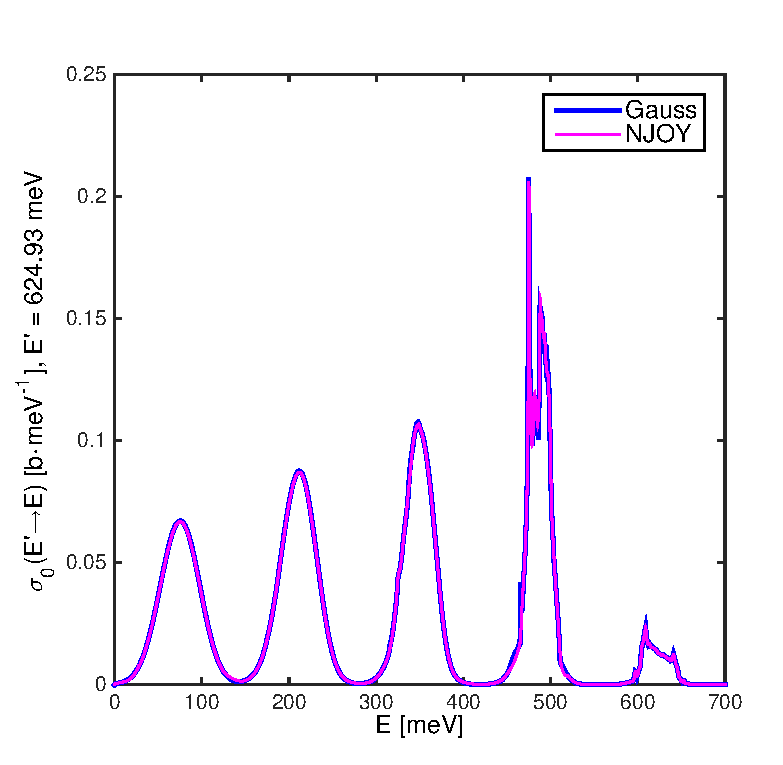
\includegraphics[width=.45\linewidth]{hgd1.eps}
%		\caption{Low order example for good agreement.}
		%  \caption{A subfigure}
		\label{fg:hgd1}}
	~
	\subfigure[Graphite]{
%		\centering
		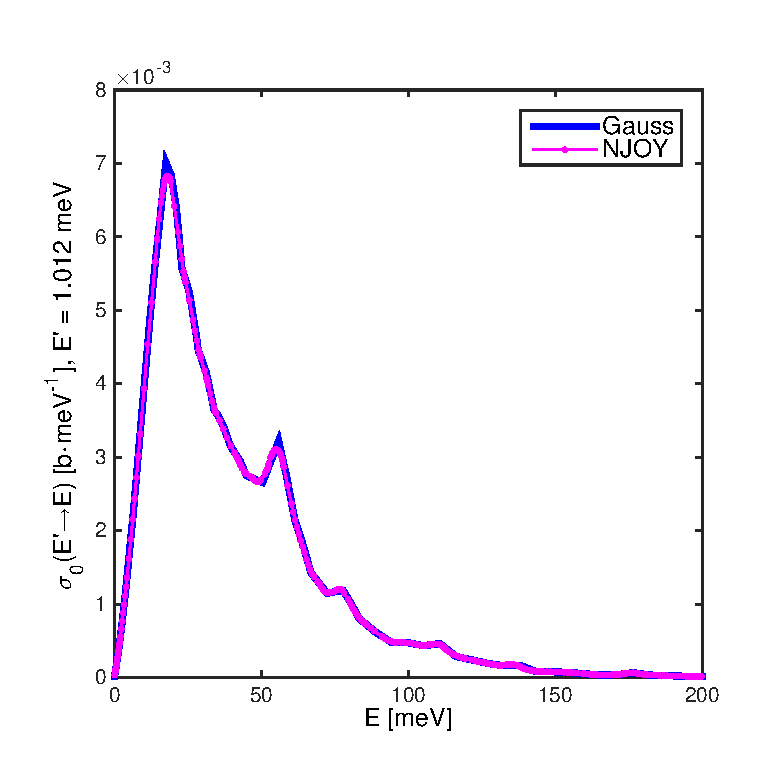
\includegraphics[width=.45\linewidth]{cgd1.eps}
%		\caption{High order example for good agreement.}
		%  \caption{A subfigure}
		\label{fg:cgd1}}
	\caption{Examples of good agreement, in the graph norm, for low order moments between codes for H in \zh~and graphite.}
	\label{fg:gdsab1}
\end{figure}

\begin{figure}[ht!]
	\centering
	\subfigure[H in \zh]{
%		\centering
		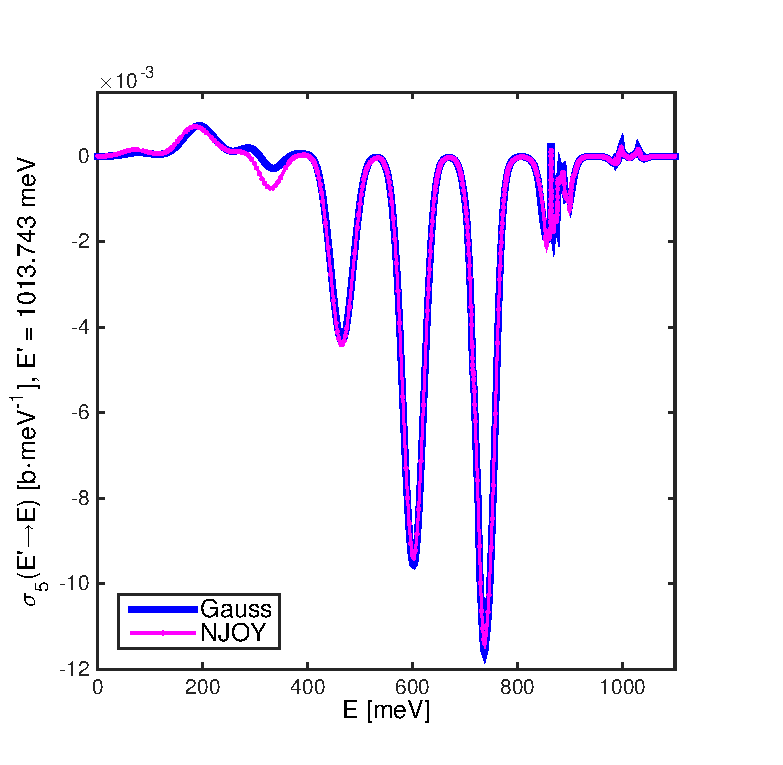
\includegraphics[width=.45\linewidth]{hgd2.eps}
%		\caption{Low order example for good agreement.}
		%  \caption{A subfigure}
		\label{fg:hgd2}}
	~
	\subfigure[Graphite]{
%		\centering
		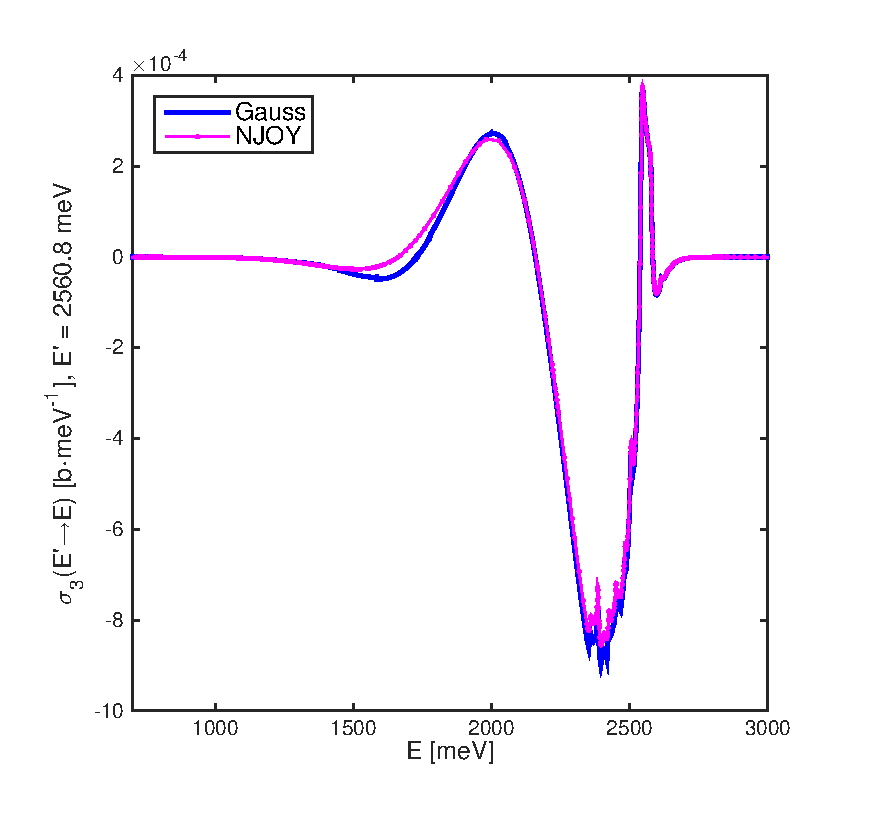
\includegraphics[width=.45\linewidth]{cgd2.eps}
%		\caption{High order example for good agreement.}
		%  \caption{A subfigure}
		\label{fg:cgd2}}
	\caption{Examples of good agreement, in the graph norm, for higher order moments between codes for H in \zh~and graphite.}
	\label{fg:gdsab2}
\end{figure}

When the incident energy is low enough, the high order moments do not agree between the Gauss quadrature and EPC results from NJOY99 as illustrated by the example shown in Figure~\ref{fg:bdsab1}.
\begin{figure}[ht!]
	\centering
	\subfigure[H in \zh]{
%		\centering
		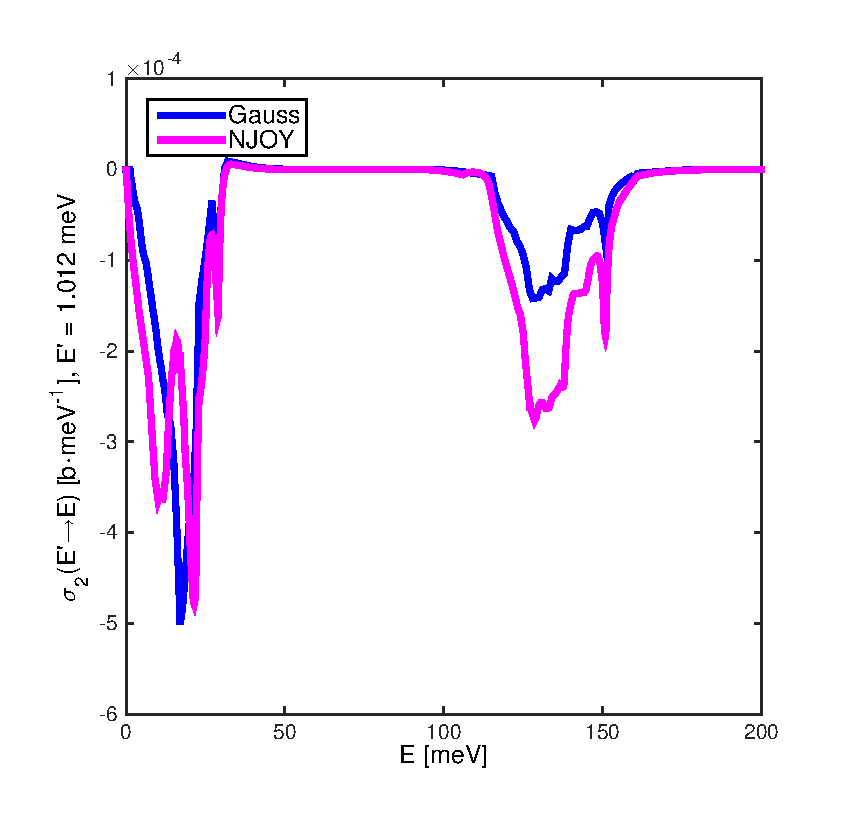
\includegraphics[width=.45\linewidth]{hbd1.eps}
%		\caption{Low order example for good agreement.}
		%  \caption{A subfigure}
		\label{fg:hbd1}}
	~
	\subfigure[Graphite]{
%		\centering
		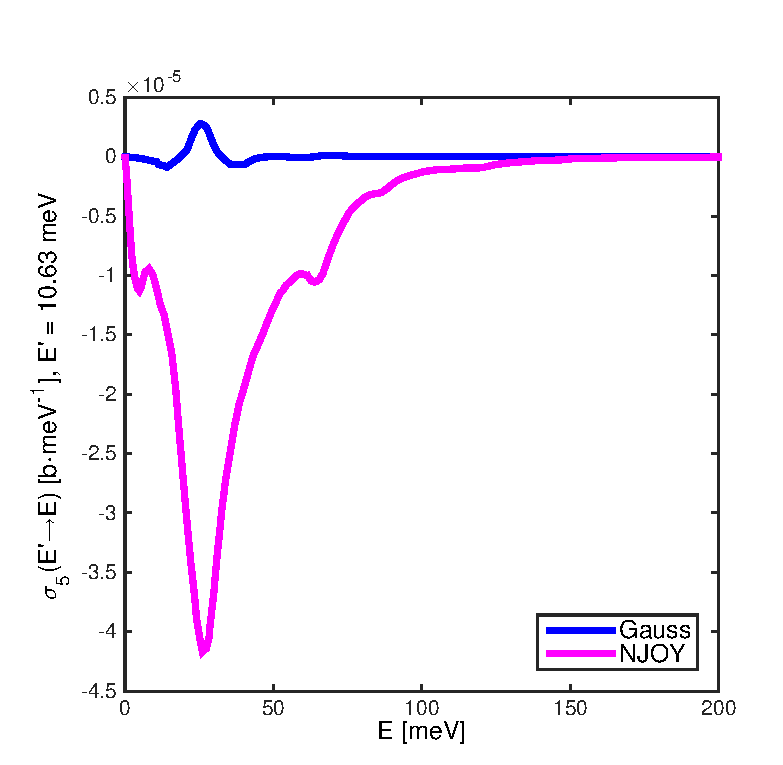
\includegraphics[width=.45\linewidth]{cbd1.eps}
%		\caption{High order example for good agreement.}
		%  \caption{A subfigure}
		\label{fg:cbd1}}
	\caption{Examples of poor agreement, in the graph norm, for higher order moments between codes for H in \zh~and graphite.}
	\label{fg:bdsab1}
\end{figure}

%\tcr{\section{A manufactured example}}
%
%	
%	\textcolor{blue}{A simple example is by using the following double differential scattering cross section assuming unitary zeroth moment (i.e.,\,$\sigma_0=1$):
%		\begin{equation}
%		\sigma(E'\to E,\mu)=\frac{2}{23}\left[1+\frac{19}{1+\exp\left(K(\mu+0.25)\right)}-\frac{19}{1+\exp\left(K(\mu-0.25)\right)}\right],\quad\mu\in[-1,\,1],\,K=1\e{10}
%		\end{equation}
%This function leads to an anisotropic angular distribution as shown in Figure\ \ref{f:ani}.\ We compare 16-bin EPC with 16-point Gaussian integration for different orders of Legendre moments in Table\,\ref{tb:manu}\ by using adaptive integration function with Gauss-Kronrod rule in {\tt MATLAB}\ as a reference\cite{matlab}. EPC method generates good results in low orders, but Gaussian integration with 16 quadrature points presents relatively poor results for $l\leq 2$. When increasing the order, EPC begins to produce larger errors than Gaussian integration.
%		}
%
%\begin{figure}
%	\centering
%	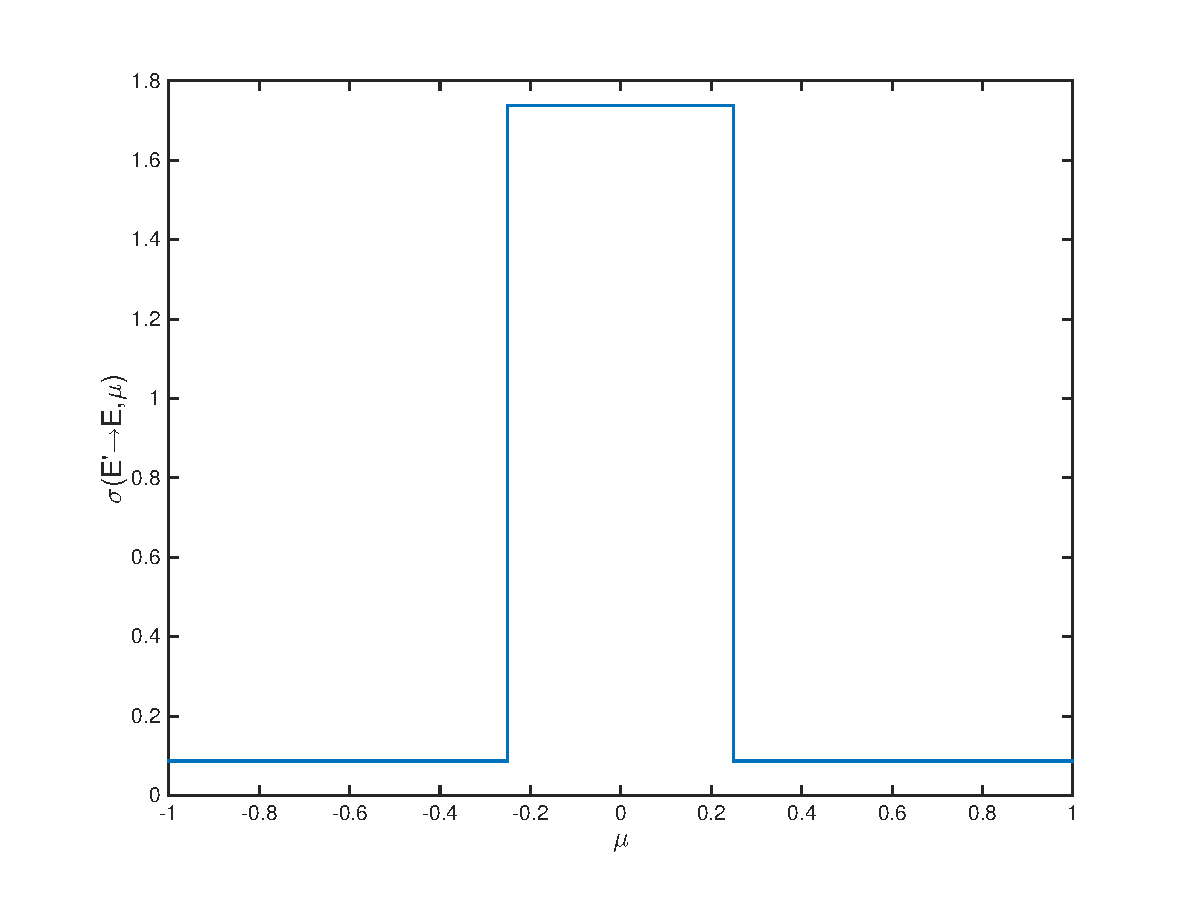
\includegraphics[width=.65\linewidth]{fani.eps}
%	\caption{Anisotropic scattering cross section example.}
%	\label{f:ani}
%\end{figure}
%
%\begin{table}[h]
%	\centering
%	\caption{Comparison between EPC and Gaussian integration}
%	\label{tb:manu}
%	\begin{tabular}{|c|c|c|c|c|c|c|c|c|c|}
%		%\label{tb:1}
%		\hline
%		Methods & $\sigma_0$ & $\sigma_1$ & $\sigma_2$ & $\sigma_3$ & $\sigma_4$ & $\sigma_5$ & $\sigma_6$ & $\sigma_7$ & $\sigma_8$ \\
%		\hline
%		Ref. &  1      & 0 & -0.3872 & 0 & 0.2481 & 0 & -0.1575 & 0 & 0.0888\\
%		\hline
%		EPC &   1      & 0 & -0.3868 & 0 & 0.2097 & 0 & -0.1594 & 0 & 0.1307\\
%		\hline
%		Gauss & 0.7999 & 0 & -0.3045 & 0 & 0.2138 & 0 & -0.1595 & 0 & 0.1118\\
%		\hline
%		
%	\end{tabular}
%	
%\end{table}
\section{Analytical derivation of continuous-energy Legendre moments and methods comparison}
Before generating MG Legendre moments, one needs to calculate the thermal scattering law based on the phonon spectrum\footnote{The details of this derivation implemented will not be repeated in this paper. The interested reader can find these derivations and algorithms for calculating the scattering law in Ref.~\cite{glasstone}.}. It is not possible to tell whether the discrepancies shown in the above figures come from the process of doing angular integration with either Gauss quadrature or EPC method or from the numerical process of synthesizing the scattering law from the phonon spectrum.

In order to remove this ambiguity and provide benchmark solutions, it is necessary to use the scattering laws which have analytic and simple forms minimizing errors from the numerical scattering law\footnote{Further details regarding numerically synthesized scattering law may be found in Ref.~\cite{Macf}}. Therefore, we use the free gas model, which has been widely used in transport calculations. Furthermore, the derivation of the differential scattering cross section ($0^\mathrm{th}$~order moment) of such model has been known for decades, it is reasonable to hypothesize the existence of analytical forms of the Legendre moments with order larger than zero. Indeed these forms exist but they are lengthy, as we show below.

A free gas has a scattering kernel of Dirac delta function, which results in the scattering law given by:
\begin{equation}\label{law}
\law=\frac{1}{\sqrt{4\pi\alpha}}\exp\left(-\frac{(\alpha+\beta)^2}{4\alpha}\right)
\end{equation}

The typical derivation of free gas scattering cross section is based on the analysis in the two-body scattering in the centered mass model (CM) \cite{glasstone}. It is difficult, though likely possible, to extend such analysis to other orders. 
Fortunately, we may obtain higher order scattering scattering moments with the scattering law shown in Eq.~\eqref{law}~without the CM model.
\subsection{Derivation of Legendre moments for free gas model}
In our derivation, we use some substitutions in Eq.~\eqref{law} to make the presentation more straightforward:
%are needed to suit the symbolic {\tt Mathematica}l package {\tt Mathematica}~\footnote{The transformation would not be unique.}.~If we define:
\begin{equation}\label{parts}
a\equiv\frac{E+E'}{AkT}\mathrm{,}\qquad\qquad b\equiv\frac{2\sqrt{EE'}}{AkT},\qquad\mathrm{and}\qquad c\equiv\frac{\hat{\sigma}_\mathrm{b}}{4kT\sqrt{4\pi}}\sqrt{\frac{E}{E'}}.
\end{equation}
We then substitute corresponding parts of Eq.~\eqref{law}~with Eq.~\eqref{parts} and plug it into Eq.~\eqref{ddx}, one arrives at the functional form of double differential scattering cross section:
\begin{equation}
\sigma(a,b,c,\beta,\mu)=\frac{c}{\sqrt{a-b\mu}}\exp\left(-\frac{(\beta+a-b\mu)^2}{4(a-b\mu)}\right).
\end{equation}
Therefore the moments can be rewritten as:
\begin{equation}
\sigma_l(a,b,c,\beta)=\int\limits_{-1}^{1}d\mu\frac{c}{\sqrt{a-b\mu}}\exp\left(-\frac{(\beta+a-b\mu)^2}{4(a-b\mu)}\right)P_l(\mu).
\end{equation}
With a few more steps, we obtain the expression we use for this paper:
\begin{equation}
\sigma_l(a,b,c,\beta)=\int\limits_{\sqrt{a-b}}^{\sqrt{a+b}}du\frac{2c}{b}\exp\left(-\frac{1}{4}\left(u+\frac{\beta}{u}\right)^2\right)P_l\left(\frac{b-u^2}{a}\right).
\end{equation}

The computer algebra software {\tt Mathematica} can take this expression into symbolic calculations for any order of Legendre polynomials\cite{mathematica9}. %The results are in forms of functionals.
Here we show the derived expression for the zeroth order moment in Eq.~\eqref{sig0abc}~and the first order moment in Eq.~\eqref{sig1abc}. The expressions for moments 2 and higher are too lengthy to reproduce here, but they can be handled by {\tt Mathematica}:
\begin{align}\label{sig0abc}
\sigma_0(a,b,c,\beta)&=\frac{c}{b}e^{-\frac{\beta+|\beta|}{2}}\sqrt{\pi}\left\{-\mathrm{erf}\left(\frac{a-b-|\beta|}{2\sqrt{a-b}}\right)+\mathrm{erf}\left(\frac{a+b-|\beta|}{2\sqrt{a+b}}\right)\right.\nonumber\\
&\left.+e^{|\beta|}\left[-\mathrm{erf}\left(\frac{a-b+|\beta|}{2\sqrt{a-b}}\right)+\mathrm{erf}\left(\frac{a+b+|\beta|}{2\sqrt{a+b}}\right)\right]\right\}
\end{align}

\begin{align}\label{sig1abc}
\sigma_1(a,b,c,\beta)&=\frac{\sqrt{\pi}c}{b^2}e^{-\frac{1}{2} \left(|\beta|+\beta
		\right)} \left\{\left(a-|\beta|-2\right) \mathrm{erf}\left(\frac{a+b-|\beta|}{2 \sqrt{a+b}}\right)\right.\nonumber\\
	&\left.
	+\left(a+|\beta|-2\right)
	e^{|\beta|}
	\left[\mathrm{erf}\left(\frac{a+b+|\beta|}{2 \sqrt{a+b}}\right)-1+e^{-|\beta|}\right]
	\right.\nonumber\\
	&\left.+4\sqrt{\frac{a+b}{\pi}}
	e^{-\frac{1}{4(a+b)}\left(a+b-|\beta|\right)^2} \right\}\nonumber\\ %________________
	&-\frac{\sqrt{\pi}c}{b^2}e^{\frac{1}{4} \left(
		-\frac{\beta
			^2}{a-b}-a-2 |\beta|-2 \beta \right)}
	\left\{\left(a-|\beta|-2\right) \mathrm{erf}\left(\frac{a-b-|\beta|}{2
		\sqrt{a-b}}\right)\right.\\
	&\left.+ \left(a+|\beta|-2\right)
	e^{|\beta|}\left[
	\mathrm{erf}\left(\frac{a-b+|\beta|}{2 \sqrt{a-b}}\right)+1-e^{|\beta|}\right]\right.\nonumber\\
	&\left.+4
	\sqrt{\frac{a-b}{\pi}} e^{-\frac{1}{4(a-b)} \left(a-b-|\beta|\right)^2}\right\}\nonumber
\end{align}


Using the expressions of $a$,~$b$,~$c$~and $\beta$~in Eq.~\eqref{sig0abc} and \eqref{sig1abc}, one obtains the expressions for moments in functions of $E$,~$E'$~and $T$. For example, $\sigma_0(E'\to E)$ is given by:
%\begin{equation}

%\end{equation}
%\begin{align}\label{eq:formerfreegas}
%%\sigma_0(E'\to E) & =\frac{\sigma_\mathrm{f}}{E'}\frac{\eta^2}{2}\left\{\exp\left(\epkt-\ekt\right)\left[\erf\left(\eta\sqrt{\epkt}-\rho\sqrt{\ekt}\right)\\
%%\quad& \pm\left(\eta\sqrt{\epkt}+\rho\sqrt{\ekt}\right)\right]+\left[\erf\left(\eta\sqrt{\ekt}-\rho\sqrt{\epkt}\right)\\
%%\quad & \mp\left(\eta\sqrt{\ekt}+\rho\sqrt{\epkt}\right)\right]\right\},
%\sigma_0(E'\to E) & =\frac{\sigma_\mathrm{f}}{E'}\frac{\eta^2}{2}\Bigg\{\exp\left(\epkt-\ekt\right)\Bigg[\erf\left(\eta\sqrt{\epkt}-\rho\sqrt{\ekt}\right)\nonumber\\
%& \pm\left(\eta\sqrt{\epkt}+\rho\sqrt{\ekt}\right)\Bigg]+\Bigg[\erf\left(\eta\sqrt{\ekt}-\rho\sqrt{\epkt}\right)\\
%& \mp\left(\eta\sqrt{\ekt}+\rho\sqrt{\epkt}\right)\Bigg]\Bigg\}\nonumber,
%\end{align}
\begin{multline}\label{eq:formerfreegas}
%\sigma_0(E'\to E) & =\frac{\sigma_\mathrm{f}}{E'}\frac{\eta^2}{2}\left\{\exp\left(\epkt-\ekt\right)\left[\erf\left(\eta\sqrt{\epkt}-\rho\sqrt{\ekt}\right)\\
%\quad& \pm\left(\eta\sqrt{\epkt}+\rho\sqrt{\ekt}\right)\right]+\left[\erf\left(\eta\sqrt{\ekt}-\rho\sqrt{\epkt}\right)\\
%\quad & \mp\left(\eta\sqrt{\ekt}+\rho\sqrt{\epkt}\right)\right]\right\},
\sigma_0(E'\to E)  =\frac{\sigma_\mathrm{f}}{E'}\frac{\eta^2}{2}\Bigg\{\exp\left(\epkt-\ekt\right)\Bigg[\erf\left(\eta\sqrt{\epkt}-\rho\sqrt{\ekt}\right)\\
\pm\left(\eta\sqrt{\epkt}+\rho\sqrt{\ekt}\right)\Bigg]+\Bigg[\erf\left(\eta\sqrt{\ekt}-\rho\sqrt{\epkt}\right)\\
 \mp\left(\eta\sqrt{\ekt}+\rho\sqrt{\epkt}\right)\Bigg]\Bigg\},
\end{multline}
%\end{equation}
where
\begin{equation}
\eta\equiv\frac{A+1}{2\sqrt{A}},\qquad\rho\equiv\frac{A-1}{2\sqrt{A}}\qquad\mathrm{and}\qquad\sigma_\mathrm{f}=\hat{\sigma}_\mathrm{b}\left(\frac{A}{A+1}\right)^2,
\end{equation}
and the upper (lower) signs are to be used if $E'<E$~($E'>E$). Eq.~\eqref{eq:formerfreegas}~is exactly what previous researchers derived through analyses in CM system \cite{glasstone}. This agreement of the results from distinct analysis process demonstrates the efficacy of the functional derivation used in this paper. Our derivations in this paper actually avoid the complexity of analyses in CM system with a concomitant increase in algebraic complexity that can be handled by computer algebra software.
\subsection{Continuous-energy results comparison}
With the derived analytical expressions in functional forms, one could easily calculate the continuous-energy (CE) moments. % with simple transformations of the formulas  from functional to functions. 
We have observed that for all energy ranges, the low order moments, i.e.~$0^\mathrm{th}$~to~$3^\mathrm{rd}$, agree well, in the viewgraph norm for results from  EPC and Gauss quadrature, as demonstrated in Figure~\ref{fg:gde}.


\begin{figure}[ht!]
	\centering
	\subfigure[Zeroth Order]{
%		\centering
		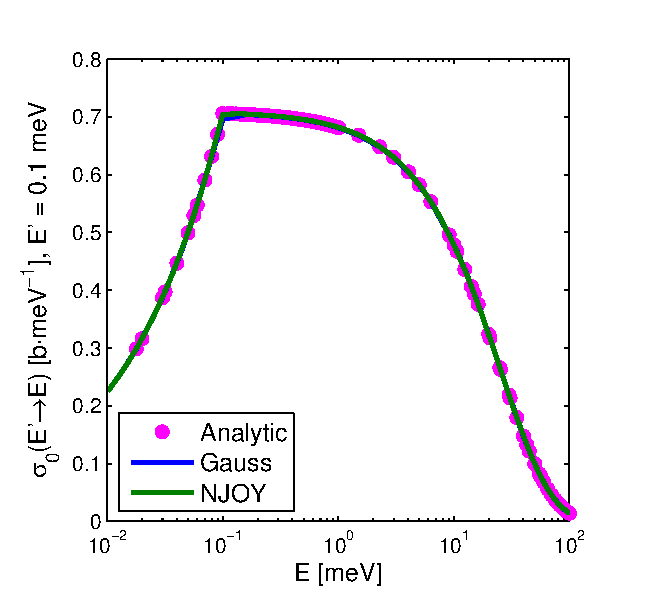
\includegraphics[width=.45\linewidth]{gd1.eps}
%		\caption{Low order example for good agreement.}
		%  \caption{A subfigure}
		\label{fg:gd1}}
	~
	\subfigure[Third Order]{
%		\centering
		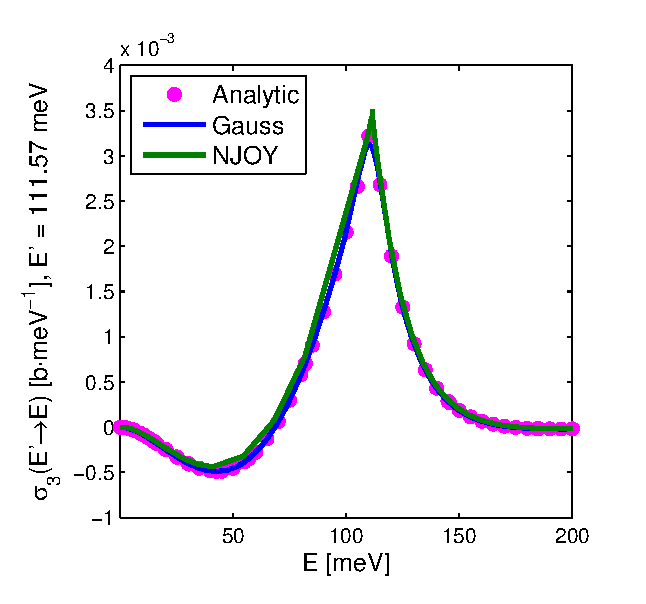
\includegraphics[width=.45\linewidth]{gd2.eps}
%		\caption{High order example for good agreement.}
		%  \caption{A subfigure}
		\label{fg:gd2}}
	\caption{Examples of good agreement in the graph norm between numerical calculations and analytical formula for two different scattering orders.}
	\label{fg:gde}
\end{figure}

Nevertheless, discrepancies occur in high order moments, which are observed to be $4^\mathrm{th}$~or higher, between EPC and analytic results, while Gauss quadrature agrees with analytical solutions. There seem to be two patterns in the discrepancies: for those low incident energy cases, such as the ones shown in Figure~\ref{fg:bdlow},~disagreement between NJOY and Gauss quadrature mainly happens in the up-scattering region (right side of the peak); for those higher energy cases with incident energy between $10$~and $100$~meV, such as the one shown in Figure~\ref{fg:bd3},~disagreement mainly occurs in the down-scattering part.~For higher energies, though discrepancies exist, the difference between codes shrink as the example illustrated in Figure~\ref{fg:bd4}. In contrast, Gauss quadrature, preserves the analytical results. Also notice that in Figure\,\ref{fg:bdlow}\,the EPC results have the opposite sign of the analytic results. %\textcolor{red}{The disagreement between EPC in NJOY and analytical results somehow demonstrate our opinion on EPC illustrated in Section\ \ref{sec:epcprob}\ that using Eq.\ \eqref{e:epsfbar}}

\begin{figure}[ht!]
	\centering
	\subfigure[$\sigma_4(E'\rightarrow E)$ with $E'=0.506$~meV]{
%		\centering
		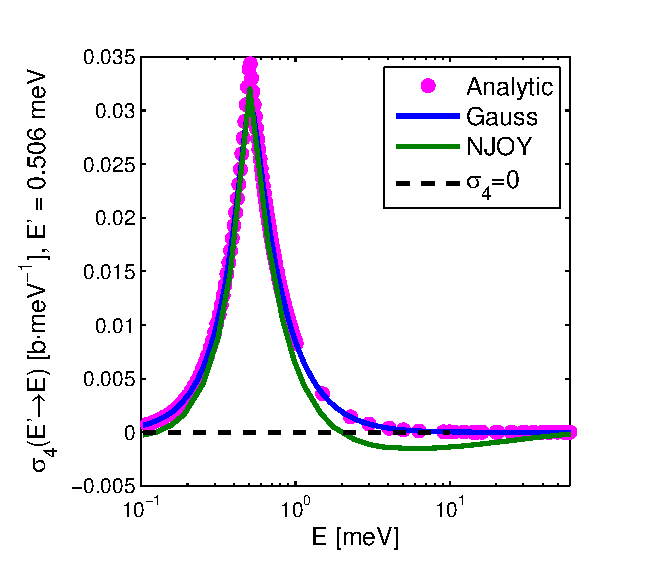
\includegraphics[width=.49\linewidth]{bd1.eps}
%		\caption{Low order example for good agreement.}
		%  \caption{A subfigure}
		\label{fg:bd1}}
	~
	\subfigure[$\sigma_5(E'\rightarrow E)$ with $E'=10.63$~meV]{
%		\centering
		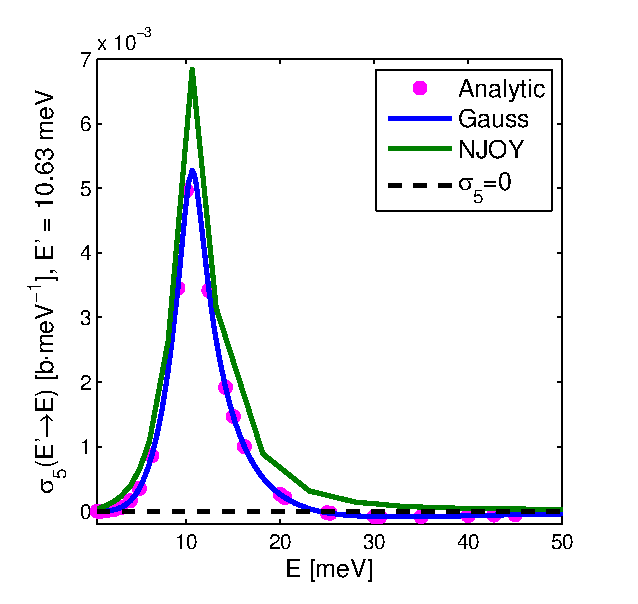
\includegraphics[width=.43\linewidth]{bd2.eps}
%		\caption{High order example for good agreement.}
		%  \caption{A subfigure}
		\label{fg:bd2}}
	\caption{At low incident energies, high order moments have disagreement between the analytic formulae and EPC for  up-scattering.}
	\label{fg:bdlow}
\end{figure}

\begin{figure}[ht!]
	\centering
	\subfigure[$\sigma_5(E'\rightarrow E)$ with $E'=56.925$~meV]{
%		\centering
		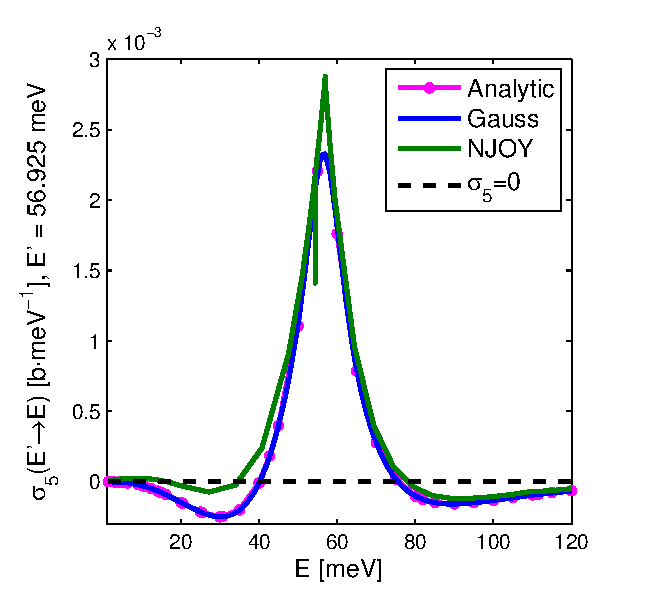
\includegraphics[width=.45\linewidth]{bd3.eps}
%		\caption{Low order example for good agreement.}
		%  \caption{A subfigure}
		\label{fg:bd3}}
	~
	\subfigure[$\sigma_5(E'\rightarrow E)$ with  $E'=111.57$~meV]{
%		\centering
		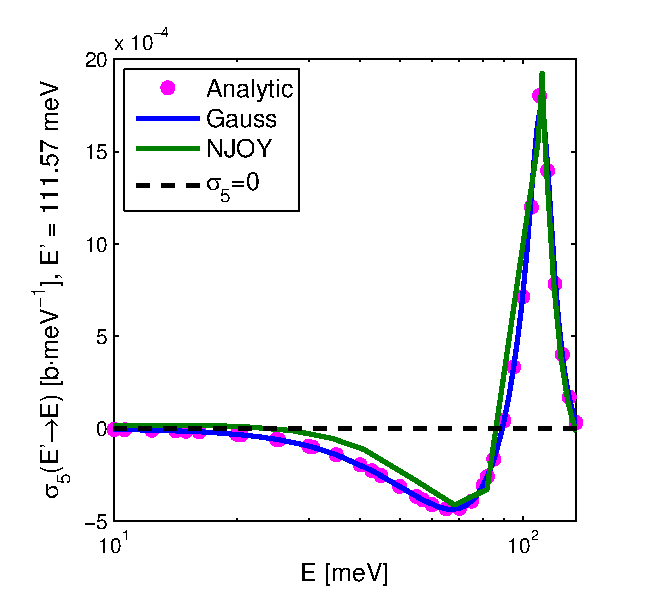
\includegraphics[width=.45\linewidth]{bd4.eps}
%		\caption{High order example for good agreement.}
		%  \caption{A subfigure}
		\label{fg:bd4}}
	\caption{At high incident energies, high order moments have disagreement between the analytic formulae and EPC for  down-scattering.}
	\label{fg:bdhigh}
\end{figure}

\section{Semi-analytic group constants}
The success in deriving analytical forms of free gas continuous-energy scattering Legendre moments enables one to develop accurate test solutions in multigroup form. We may refer to these multigroup constants as a semi-analytic benchmark since the whole process involves analytical calculations of CE moments and numerical calculations of MG moments. This will allow us to make more quantitative comparisons between the different methods.

Though EPC disagrees with analytical results for high order moments while our code agrees, it is still unclear what types of effects the discrepancies would propagate through group collapse to MG constants. Therefore, it would be critical to generate those MG constants to test results with CE moments from EPC and Gauss quadrature.

From the expressions for CE moments derived analytically, one could therefore calculate the MG Legendre moments by:
\begin{equation}\label{eq:sggtheory}
\sigma_{l,\mathrm{g'}\to\mathrm{g}}=\frac{\int\limits_{\Delta E_\mathrm{g'}}dE'\,f(E')\int\limits_{\Delta E_\mathrm{g}}dE\,\sigma_l(E'\to E)}{\int\limits_{\Delta E_\mathrm{g'}}dE'f(E')},
\end{equation}
where $f(E')$~is the weighting function. For applications, e.g.~thermal reactor simulations, a Maxwellian spectrum is chosen to approximate the exact scalar flux. In our calculations the weighting function in the thermal region is set to be the Maxwellian spectrum with a temperature of $296$~K. We choose the group boundaries to be: $0.596$,~$10.63$,~$56.925$~and $145.728$~meV, which are from the energy grids in GROUPR module of NJOY\cite{NJOY}.

\subsection{2D trapezoidal rule and error estimator}

The trapezoidal rule is used in our calculations as a reference. %Formulations in  this paper we use forward numbering of group numbers to keep the consistency with NJOY's convention, i.e.~the group with highest energy will be numbered as Group 1 while the one with lowest energy will be numbered Group G. 
If we define terms in Eq.~\eqref{eq:sggtheory}~by:
\begin{equation}
\fgp\equiv\int\limits_{\Delta\egp}dE'f(E')\qquad\mathrm{and}\qquad g(E',E)\equiv f(E')\sigma_l(E'\to E),
\end{equation}
Eq.~\eqref{eq:sggtheory}~can be rewritten as:
\begin{equation}\label{eq:sggnew}
\sgg=\frac{1}{\fgp}\int\limits_{\egp}^{\egpo} dE'\int\limits_{\eg}^{\ego} dE\,g(E',E).
\end{equation}

With the trapezoidal rule, Eq.~\eqref{eq:sggnew}~can be approximated by:
\begin{align}\label{eq:sggapp}
\sgg&\approx\frac{1}{\fgp}\int\limits_{\egp}^{\egpo} dE'\frac{h}{2}\sum\limits_{\mathrm{i=}1}^{N}\left[g(E',E_\mathrm{i})+g(E',E_\mathrm{i+1})\right]\nonumber\\
 &\approx\frac{h'h}{4\fgp}\sum\limits_{\mathrm{j=}1}^{N'}\Bigg\{\sum\limits_{\mathrm{i=}1}^{N}\left[g\left(E'_\mathrm{j+1},E_\mathrm{i}\right)+g\left(E'_\mathrm{j+1},E_\mathrm{i+1}\right)\right]\\
 &\quad+\sum\limits_{\mathrm{i=}1}^{N}\left[g\left(E'_\mathrm{j},E_\mathrm{i}\right)+g\left(E'_\mathrm{j},E_\mathrm{i+1}\right)\right]\Bigg\}\nonumber,
\end{align}
where energy grids are assumed uniform for both incident energy and outgoing energy, and $h'$~and $h$~are energy corresponding intervals and $N'$~and $N$~are corresponding number of intervals in the trapezoidal rule.

\subsection{Error estimator for 2D trapezoidal rule}
In terms of semi-analytic benchmark, we aim to reduce the error induced by introducing numerical integration in group collapse and preserve an analyst-defined precision. Therefore, it is necessary to develop an appropriate error estimator to indicate the precision of the semi-analytic results and use this to guide the integration.

Given that we desire high accuracy benchmarks, we therefore assume fine grids will be used for both incident and secondary energies. Denote the error by $\epsilon$~and the true moments (infinite precision) by $\sigma^{\mathrm{true}}_{l,\mathrm{g'}\to \mathrm{g}}$,~the error can be written as:
\begin{align}\label{error1}
\epsilon&=\sgg-\sigma^{\mathrm{true}}_{l,\mathrm{g'}\to \mathrm{g}}\nonumber\\
&\approx\frac{1}{\fgp}\int\limits_{\egp}^{\egpo}dE'\Bigg\{\frac{h}{2}\sum\limits_{\mathrm{i=}1}^N\left[g(E',E_\mathrm{i})+g(E',E_\mathrm{i+1})\right]-\int\limits_{\eg}^{\ego}dE\,g(E',E)\Bigg\},%\\
%&=\frac{1}{\fgp}\int\limits_{\egp}^{\egpo}dE'\sum\limits_{\mathrm{i=}1}^N\Bigg\{\frac{h}{2}\left[g(E',E_\mathrm{i})+g(E',E_\mathrm{i+1})\right]-\int\limits_{E_\mathrm{i}}^{E_\mathrm{i+1}}dE\,g(E',E)\Bigg\}\nonumber.
\end{align}
this expression is approximate because the $g'$ integral is continuous instead of discrete.
For functions having second-order derivatives over the secondary energy range $(E_\mathrm{i},E_\mathrm{i+1}),\mathrm{i}=1,\cdots,N$, there exists an energy $\zeta_\mathrm{i}\in[E_\mathrm{i},E_\mathrm{i+1}]$,~such that the error of trapezoidal rule could be given as \cite{numana1}:
\begin{equation}\label{eq:interm1}
\frac{h}{2}\left[g(E',E_\mathrm{i})+g(E',E_\mathrm{i+1})\right]-\int\limits_{E_\mathrm{i}}^{E_\mathrm{i+1}}dEg(E',E)=\frac{h^3}{12}\frac{\partial^2}{\partial E^2}g(E',\zeta_\mathrm{i}).
\end{equation}
Plugging Eq.~\eqref{eq:interm1}~into Eq.~\eqref{error1},~one obtains:
\begin{equation}
\epsilon\approx\frac{1}{\fgp}\int\limits_{\egp}^{\egpo}dE'\sum\limits_{\mathrm{i=}1}^{N}\frac{h^3}{12}\frac{\partial^2}{\partial E^2}g(E',\zeta_\mathrm{i}),
\end{equation}
and with the assumption of fine energy grid, one may obtain the approximation:
\begin{equation}
\sum\limits_{\mathrm{i=1}}^{N}h\frac{\partial^2}{\partial E^2}g(E',\zeta_\mathrm{i})\approx\int\limits_{E_\mathrm{g}}^{E_\mathrm{g+1}}dE\frac{\partial^2}{\partial E^2}g(E',E)=\frac{\partial}{\partial E}\left[g(E',\ego)-g(E',\eg)\right].
\end{equation}
Then the error can be approximated by:
\begin{align}\label{errorfinal}
\epsilon_{\mathrm{g'}\to\mathrm{g}}&\approx\frac{1}{\fgp}\int\limits_{\egp}^{\egpo}dE'\frac{h^2}{12}\frac{\partial}{\partial E}\left[g(E',\ego)-g(E',\eg)\right]\nonumber\\
&\approx\frac{h^2h'}{24\fgp}\frac{\partial}{\partial E}\sum\limits_{\mathrm{j=}1}^{N'}\bigg[g(E'_\mathrm{j+1},\ego)+g(E'_\mathrm{j},\ego)\\
& \qquad -g(E'_\mathrm{j+1},\eg)-g(E'_\mathrm{j},\eg)\bigg]\nonumber.
\end{align}
The error given by Eq.~\eqref{errorfinal}~is computable. With this, a modeler could calculate the MG Legendre moments to a desired precision. We use this formula to help decide when our benchmark calculations are converged.% with a few iterations on changing energy grids based on results from Eq.~\eqref{eq:sggapp}~and Eq.~\eqref{errorfinal}. 
%Furthermore, from Eq.~\eqref{errorfinal},~one would observe the error is second order about the variable firstly integrated with. Observations from thermal treatments (cite NJOY) suggest the scattering moments varies fast versus secondary energy but slowly versus incident energy. In the end, it would suggest integrating the CE Legendre moments over the fast varying secondary energy first to preserve second-order accuracy and then over the slowly varying incident energy to preserve the first-order accuracy.\textcolor{red}{Clear? well I confused myself.}
\subsection{MG benchmark results}

The trapezoidal rule will be used to integrate the EPC and the Gauss quadrature CE Legendre moments and then compared to the semi-analytic MG constants. NJOY has this integration  built in, and we have included it in our implementation of the Gauss quadrature code.  The refinement criteria for the integration is based on the relative change in the integral when an interval is halved. That is, if the integral changes by a relative amount smaller than a given tolerance when  an interval is halved, the integral on that interval is said to have converged, otherwise the integral is halved again. We set this relative error bound in NJOY and our Gauss quadrature code to be $10^{-8}$. 
For the benchmark solution based on the analytic formula, we refine until our error estimate is below this same tolerance.  %The actual errors after auto energy grid refinement reach a maximum of $3.8\times10^{-9}$. 

Table~\ref{tb:1}~shows the group structure and corresponding ordering. Table~\ref{tb:2}~presents semi-analytic MG thermal scattering Legendre moments for H-1 free gas model to six digits.
\begin{table}[h]
\centering
\caption{Group structure and numbering}
\label{tb:1}
\begin{tabular}{|c|c|}
%\label{tb:1}
\hline
Group bounds [eV] & Group number\\
\hline
$5.06\e{-4}-1.063\e{-2}$ &  1\\
\hline
$1.063\e{-2}-5.6925\e{-2}$ & 2\\
\hline
$5.6925\e{-2}-1.45728\e{-1}$ & 3\\
\hline

\end{tabular}

\end{table}

\begin{table}[h]

\centering
\caption{MG semi-analytic benchmark for H-1 free gas thermal scattering Legendre moments (units: barns)}\normalsize
\label{tb:2}
\scriptsize
\begin{adjustwidth}{-0.5cm}{}
\begin{tabular}{|c|c|c|c|c|c|c|c|}
\hline
\multicolumn{2}{|c|}{Group No.} & \multicolumn{6}{c|}{Legendre orders}\\
\hline
In & out & 0 & 1 & 2 & 3 & 4 & 5\\ 
\hline
1 & 1 &  $1.43706\e{1}$  &  $4.00022$  &  $1.79315$  &  $1.02783$  &  $6.67912\e{-1}$  &  $4.68931\e{-1}$\\
\hline
1 & 2 &  $3.17180\e{1}$  &  $6.13864$  &  $1.37200$  &  $4.35582\e{-1}$  &  $1.88328\e{-1}$  &  $1.00273\e{-1}$\\
\hline
1 & 3 &  $5.97642$  &  $6.37686\e{-1}$  &  $-6.09528\e{-2}$  &  $-4.65253\e{-2}$  &  $-1.51390\e{-2}$  &  $-4.13017\e{-3}$\\
\hline
2 & 1 &  $3.56328$  &  $6.89895\e{-1}$  &  $1.54164\e{-1}$  &  $4.89546\e{-2}$  &  $2.11740\e{-2}$  &  $1.12793\e{-2}$\\
\hline
2 & 2 &  $1.99269\e{1}$  &  $7.93879$  &  $3.25486$  &  $1.60606$  &  $9.31671\e{-1}$  &  $6.02335\e{-1}$\\
\hline
2 & 3 &  $5.71948$  &  $2.09064$  &  $4.64251\e{-1}$  &  $1.88725\e{-2}$  &  $-6.08646\e{-2}$  &  $-5.86812\e{-2}$\\
\hline
3 & 1 &  $1.21398$  &  $1.29533\e{-1}$  &  $-1.23800\e{-2}$  &  $-9.45027\e{-3}$  &  $-3.07513\e{-3}$  &  $-8.38978\e{-4}$\\
\hline
3 & 2 &  $1.03477\e{1}$  &  $3.78375$  &  $8.40005\e{-1}$  &  $3.42297\e{-2}$  &  $-1.10010\e{-1}$  &  $-1.06080\e{-1}$\\
\hline
3 & 3 &  $1.14679\e{1}$  &  $7.16999$  &  $3.62659$  &  $1.74074$  &  $8.79259\e{-1}$  &  $4.87835\e{-1}$\\
\hline
\end{tabular}
\end{adjustwidth}
\end{table}
\subsection{Comparison of Gauss quadrature and EPC}
In order to test the efficacy of the Gauss quadrature in this application, we generated MG data with group structure given in Table~\ref{tb:1}~with 8 quadrature points for the angular integration. The results are shown in Table~\ref{tb:8pt}. Correspondingly, Table~\ref{tb:njoy}~shows results from NJOY with EPC method. The relative errors estimated with benchmark results are shown in Table~\ref{tb:8err}~and~\ref{tb:njoyerr},~respectively\footnote{In this paper, those points with an error $<10\%$,~$\geq10\%\mathrm{~and~}\leq20\%$,~$\geq20\%\mathrm{~and~}\leq100\%$~and $>100\%$~are marked green, cyan, yellow and red in the error tables, respectively.}.

\begin{table}[h]
\centering
\caption{MG Legendre moments with 8-point Gauss quadrature (units: barns)}\normalsize
\label{tb:8pt}
\scriptsize
\begin{adjustwidth}{-0.5cm}{}
\begin{tabular}{|c|c|c|c|c|c|c|c|}
\hline
\multicolumn{2}{|c|}{Group No.} & \multicolumn{6}{c|}{Legendre orders}\\
\hline
In & out & 0 & 1 & 2 & 3 & 4 & 5\\ 
\hline
1 & 1 & $1.41319\e{1}$ & $3.82428$ & $1.62851$ & $8.64824\e{-1}$ & $5.02628\e{-1}$ & $2.97924\e{-1}$\\
\hline
1 & 2 & $3.17333\e{1}$ & $6.13694$ & $1.37281$ & $4.32054\e{-1}$ & $1.80085\e{-1}$ & $8.78393\e{-2}$\\
\hline
1 & 3 & $5.99056$ & $6.39633\e{-1}$ & $-6.04103\e{-2}$ & $-4.69379\e{-2}$ & $-1.54457\e{-2}$ & $-4.27289\e{-3}$\\
\hline
2 & 1 & $3.58321$ & $6.98149\e{-1}$ & $1.57518\e{-1}$ & $4.95620\e{-2}$ & $2.05008\e{-2}$ & $9.90328\e{-3}$\\
\hline
2 & 2 & $1.97660\e{1}$ & $7.74602$ & $3.07471$ & $1.43507$ & $7.59176\e{-1}$ & $4.23155\e{-1}$\\
\hline
2 & 3 & $5.73372$ & $2.09659$ & $4.81762\e{-1}$ & $4.06129\e{-2}$ & $-3.87402\e{-2}$ & $-3.71309\e{-2}$\\
\hline
3 & 1 & $1.28578$ & $1.41513\e{-1}$ & $-1.13032\e{-2}$ & $-9.78833\e{-3}$ & $-3.37195\e{-3}$ & $-9.86717\e{-4}$\\
\hline
3 & 2 & $1.09501\e{1}$ & $4.11686$ & $1.04450$ & $1.74476\e{-1}$ & $-7.91058\e{-3}$ & $-2.87346\e{-2}$\\
\hline
3 & 3 & $1.12774\e{1}$ & $6.94947$ & $3.42865$ & $1.57561$ & $7.38958\e{-1}$ & $3.62634\e{-1}$\\
\hline
\end{tabular}
\end{adjustwidth}
\end{table}

\begin{table}[h]
\centering
\caption{MG Legendre moments from NJOY with EPC angular integration (units: barns)}\normalsize
\label{tb:njoy}
\scriptsize
\begin{adjustwidth}{-0.5cm}{}
\begin{tabular}{|c|c|c|c|c|c|c|c|}
\hline
\multicolumn{2}{|c|}{Group No.} & \multicolumn{6}{c|}{Legendre orders}\\
\hline
In & out & 0 & 1 & 2 & 3 & 4 & 5\\ 
\hline
1 & 1 & $1.44477\e{1}$ & $3.98588$ & $1.75101$ & $1.06242$ & $5.58801\e{-1}$ & $5.69838\e{-1}$\\
\hline
1 & 2 & $3.16504\e{1}$ & $6.11118$ & $1.29710$ & $4.97870\e{-1}$ & $-4.73181\e{-2}$ & $2.64893\e{-1}$\\
\hline
1 & 3 & $5.96637$ & $6.34556\e{-1}$ & $-7.26090\e{-2}$ & $-3.93808\e{-2}$ & $-5.87373\e{-2}$ & $1.33928\e{-2}$\\
\hline
2 & 1 & $3.47224$ & $6.71202\e{-1}$ & $1.45769\e{-1}$ & $5.59090\e{-2}$ & $-5.17761\e{-3}$ & $2.89932\e{-2}$\\
\hline
2 & 2 & $1.98469\e{1}$ & $7.88170$ & $3.17702$ & $1.70674$ & $7.20382\e{-1}$ & $8.19138\e{-1}$\\
\hline
2 & 3 & $5.72965$ & $2.08205$ & $4.42168\e{-1}$ & $5.23645\e{-2}$ & $-1.27885\e{-1}$ & $-3.05660\e{-3}$\\
\hline
3 & 1 & $1.12380$ & $1.18525\e{-1}$ & $-1.37611\e{-2}$ & $-8.74872\e{-3}$ & $-1.21743\e{-2}$ & $2.07946\e{-3}$\\
\hline
3 & 2 & $1.00978\e{1}$ & $3.65736$ & $8.11960\e{-1}$ & $1.13682\e{-1}$ & $-2.16564\e{-1}$ & $-1.04113\e{-2}$\\
\hline
3 & 3 & $1.15649\e{1}$ & $7.14974$ & $3.53120$ & $1.85044$ & $7.90635\e{-1}$ & $4.73826\e{-1}$\\
\hline
\end{tabular}
\end{adjustwidth}
\end{table}

\begin{table}[h]
\centering
\caption{Relative error of MG moments with 8-point Gauss quadrature}\normalsize
\label{tb:8err}
%\scriptsize
\begin{adjustwidth}{-0.5cm}{}
\begin{tabular}{|c|c|c|c|c|c|c|c|}
\hline
\multicolumn{2}{|c|}{Group No.} & \multicolumn{6}{c|}{Legendre orders}\\
\hline
In & out & 0 & 1 & 2 & 3 & 4 & 5\\ 
\hline
1 & 1 & \cellcolor{green} $1.66\e{-2}$ & \cellcolor{green} $4.39\e{-2}$ & \cellcolor{green} $9.18\e{-2}$ & \cellcolor{cyan} $1.58\e{-1}$ & \cellcolor{yellow} $2.47\e{-1}$ & \cellcolor{yellow} $3.64\e{-1}$\\
\hline
1 & 2 & \cellcolor{green} $4.82\e{-4}$ & \cellcolor{green} $2.77\e{-4}$ & \cellcolor{green} $5.88\e{-4}$ & \cellcolor{green} $8.10\e{-3}$ & \cellcolor{green} $4.37\e{-2}$ & \cellcolor{cyan} $1.24\e{-1}$\\
\hline
1 & 3 & \cellcolor{green} $2.36\e{-3}$ & \cellcolor{green} $3.05\e{-3}$ & \cellcolor{green} $8.90\e{-3}$ & \cellcolor{green} $8.86\e{-3}$ & \cellcolor{green} $2.02\e{-2}$ & \cellcolor{green} $3.45\e{-2}$\\
\hline
2 & 1 & \cellcolor{green} $5.59\e{-3}$ & \cellcolor{green} $1.19\e{-2}$ & \cellcolor{green} $2.17\e{-2}$ & \cellcolor{green} $1.24\e{-2}$ & \cellcolor{green} $3.17\e{-2}$ & \cellcolor{cyan} $1.22\e{-1}$\\
\hline
2 & 2 & \cellcolor{green} $8.07\e{-3}$ & \cellcolor{green} $2.42\e{-2}$ & \cellcolor{green} $5.53\e{-2}$ & \cellcolor{cyan} $1.06\e{-1}$ & \cellcolor{cyan} $1.85\e{-1}$ & \cellcolor{yellow} $2.97\e{-1}$\\
\hline
2 & 3 & \cellcolor{green} $2.48\e{-3}$ & \cellcolor{green} $2.84\e{-3}$ & \cellcolor{green} $3.77\e{-2}$ & \cellcolor{red} $1.15$ & \cellcolor{yellow} $3.63\e{-1}$ & \cellcolor{yellow} $3.67\e{-1}$\\
\hline
3 & 1 & \cellcolor{green} $5.91\e{-2}$ & \cellcolor{green} $9.24\e{-2}$ & \cellcolor{green} $8.69\e{-2}$ & \cellcolor{green} $3.57\e{-2}$ & \cellcolor{green} $9.65\e{-2}$ & \cellcolor{cyan} $1.76\e{-1}$\\
\hline
3 & 2 & \cellcolor{green} $5.82\e{-2}$ & \cellcolor{green} $8.80\e{-2}$ & \cellcolor{yellow} $2.43\e{-1}$ & \cellcolor{red} $4.09$ & \cellcolor{yellow} $9.28\e{-1}$ & \cellcolor{yellow} $7.29\e{-1}$\\
\hline
3 & 3 & \cellcolor{green} $1.66\e{-2}$ & \cellcolor{green} $3.07\e{-2}$ & \cellcolor{green} $5.45\e{-2}$ & \cellcolor{green} $9.48\e{-2}$ & \cellcolor{cyan} $1.59\e{-1}$ & \cellcolor{yellow} $2.56\e{-1}$\\
\hline
\end{tabular}
\end{adjustwidth}
\end{table}

\begin{table}[h]
\centering
\caption{Relative error of MG moments from NJOY with EPC angular integration}\normalsize
\label{tb:njoyerr}
%\scriptsize
\begin{adjustwidth}{-.5cm}{}
\begin{tabular}{|c|c|c|c|c|c|c|c|}
\hline
\multicolumn{2}{|c|}{Group No.} & \multicolumn{6}{c|}{Legendre orders}\\
\hline
In & out & 0 & 1 & 2 & 3 & 4 & 5\\ 
\hline
1 & 1 & \cellcolor{green} $5.36\e{-3}$ & \cellcolor{green} $3.58\e{-3}$ & \cellcolor{green} $2.35\e{-2}$ & \cellcolor{green} $3.36\e{-2}$ & \cellcolor{green} $1.63\e{-1}$ & \cellcolor{yellow} $2.15\e{-1}$\\
\hline
1 & 2 & \cellcolor{green} $2.13\e{-3}$ & \cellcolor{green} $4.47\e{-3}$ & \cellcolor{green} $5.45\e{-2}$ & \cellcolor{cyan} $1.42\e{-1}$ & \cellcolor{red} $1.25$ & \cellcolor{red} $1.64$\\
\hline
1 & 3 & \cellcolor{green} $1.68\e{-3}$ & \cellcolor{green} $4.90\e{-3}$ & \cellcolor{cyan} $1.91\e{-1}$ & \cellcolor{cyan} $1.53\e{-1}$ & \cellcolor{red} $2.87$ & \cellcolor{red} $4.24$\\
\hline
2 & 1 & \cellcolor{green} $2.55\e{-2}$ & \cellcolor{green} $2.70\e{-2}$ & \cellcolor{green} $5.44\e{-2}$ & \cellcolor{cyan} $1.42\e{-1}$ & \cellcolor{red} $1.24$ & \cellcolor{red} $1.57$\\
\hline
2 & 2 & \cellcolor{green} $4.01\e{-3}$ & \cellcolor{green} $7.19\e{-3}$ & \cellcolor{green} $2.39\e{-2}$ & \cellcolor{green} $6.26\e{-2}$ & \cellcolor{yellow} $2.26\e{-1}$ & \cellcolor{yellow} $3.59\e{-1}$\\
\hline
2 & 3 & \cellcolor{green} $1.77\e{-3}$ & \cellcolor{green} $4.10\e{-3}$ & \cellcolor{green} $4.75\e{-2}$ & \cellcolor{red} $1.77$ & \cellcolor{red} $1.10$ & \cellcolor{yellow} $9.47\e{-1}$\\
\hline
3 & 1 & \cellcolor{green} $7.42\e{-2}$ & \cellcolor{green} $8.49\e{-2}$ & \cellcolor{cyan} $1.11\e{-1}$ & \cellcolor{green} $7.42\e{-2}$ & \cellcolor{red} $2.95$ & \cellcolor{red} $3.47$\\
\hline
3 & 2 & \cellcolor{green} $2.41\e{-2}$ & \cellcolor{green} $3.34\e{-2}$ & \cellcolor{green} $3.33\e{-2}$ & \cellcolor{red} $2.32$ & \cellcolor{yellow} $9.68\e{-1}$ & \cellcolor{yellow} $9.01\e{-1}$\\
\hline
3 & 3 & \cellcolor{green} $8.45\e{-3}$ & \cellcolor{green} $2.82\e{-3}$ & \cellcolor{green} $2.63\e{-2}$ & \cellcolor{green} $6.30\e{-2}$ & \cellcolor{cyan} $1.00\e{-1}$ & \cellcolor{green} $2.87\e{-2}$\\
\hline
\end{tabular}
\end{adjustwidth}
\end{table}

When increasing the number of quadrature points to 20, the errors in the Gauss quadrature results are reduced, as shown in Table~\ref{tb:20err}.%~In the Table~\ref{tb:20err},~the data are calculated using 20-point Gauss quadrature to carry out the angular integration. 

\begin{table}[h]
\centering
\caption{Relative error of MG moments with 20-point Gauss quadrature}\normalsize
\label{tb:20err}
%\scriptsize
\begin{adjustwidth}{-.5cm}{}
\begin{tabular}{|c|c|c|c|c|c|c|c|}
\hline
\multicolumn{2}{|c|}{Group No.} & \multicolumn{6}{c|}{Legendre orders}\\
\hline
In & out & 0 & 1 & 2 & 3 & 4 & 5\\ 
\hline
1 & 1 & \cellcolor{green} $8.39\e{-3}$ & \cellcolor{green} $1.52\e{-2}$ & \cellcolor{green} $2.56\e{-2}$ & \cellcolor{green} $4.16\e{-2}$ & \cellcolor{green} $5.77\e{-2}$ & \cellcolor{green} $7.67\e{-2}$\\
\hline
1 & 2 & \cellcolor{green} $9.87\e{-4}$ & \cellcolor{green} $2.43\e{-3}$ & \cellcolor{green} $1.27\e{-2}$ & \cellcolor{green} $3.01\e{-2}$ & \cellcolor{green} $7.09\e{-2}$ & \cellcolor{green} $7.24\e{-2}$\\
\hline
1 & 3 & \cellcolor{green} $2.36\e{-3}$ & \cellcolor{green} $3.05\e{-3}$ & \cellcolor{green} $8.91\e{-3}$ & \cellcolor{green} $8.86\e{-3}$ & \cellcolor{green} $2.02\e{-2}$ & \cellcolor{green} $3.44\e{-2}$\\
\hline
2 & 1 & \cellcolor{green} $6.01\e{-3}$ & \cellcolor{green} $1.45\e{-2}$ & \cellcolor{green} $3.27\e{-2}$ & \cellcolor{green} $4.71\e{-2}$ & \cellcolor{green} $6.50\e{-2}$ & \cellcolor{green} $5.71\e{-2}$\\
\hline
2 & 2 & \cellcolor{green} $2.05\e{-3}$ & \cellcolor{green} $8.93\e{-3}$ & \cellcolor{green} $1.71\e{-2}$ & \cellcolor{green} $2.97\e{-2}$ & \cellcolor{green} $4.86\e{-2}$ & \cellcolor{green} $6.56\e{-2}$\\
\hline
2 & 3 & \cellcolor{green} $1.85\e{-3}$ & \cellcolor{green} $3.49\e{-4}$ & \cellcolor{green} $2.70\e{-2}$ & \cellcolor{yellow} $8.89\e{-1}$ & \cellcolor{yellow} $2.65\e{-1}$ & \cellcolor{yellow} $2.40\e{-1}$\\
\hline
3 & 1 & \cellcolor{green} $5.91\e{-2}$ & \cellcolor{green} $9.25\e{-2}$ & \cellcolor{green} $8.70\e{-2}$ & \cellcolor{green} $3.58\e{-2}$ & \cellcolor{green} $9.65\e{-2}$ & \cellcolor{cyan} $1.76\e{-1}$\\
\hline
3 & 2 & \cellcolor{green} $5.91\e{-2}$ & \cellcolor{green} $9.00\e{-2}$ & \cellcolor{yellow} $2.55\e{-1}$ & \cellcolor{red} $4.35$ & \cellcolor{yellow} $9.99\e{-1}$ & \cellcolor{yellow} $7.59\e{-1}$\\
\hline
3 & 3 & \cellcolor{green} $1.22\e{-2}$ & \cellcolor{green} $2.65\e{-2}$ & \cellcolor{green} $4.55\e{-2}$ & \cellcolor{green} $7.91\e{-2}$ & \cellcolor{cyan} $1.13\e{-1}$ & \cellcolor{cyan} $1.60\e{-1}$\\
\hline
\end{tabular}
\end{adjustwidth}
\end{table}

Generally speaking, both 8-point and 20-point Gauss quadrature are comparable to EPC method for low order results (order 2 or smaller). Nevertheless, the 8-point Gauss quadrature  outperforms EPC for high order moments (Order 3 or higher) giving  smaller errors e.g.~those data in red spots (errors $>100\%$). Increasing to 20 quadrature points further reduces the errors for the high order moments as shown in Table~\ref{tb:20err}. Note that for high order moments the EPC method can give the wrong sign for the moments, e.g., $\sigma_{5,1\rightarrow 2}$.

\section{Conclusions}
\subsection{Summary}
In this paper, we began by using Gauss quadrature in synthesizing CE Legendre moments before performing group collapse. In implementations for materials with numerical scattering laws (graphite and H in \zh~in this paper), we observed agreement for low order Legendre scattering moments at low energies, and observed discrepancies between results from Gauss quadrature and NJOY results with EPC method for higher moments.

We hypothesized the discrepancies would mainly come from the distinction of angular integrations. We then derived the analytic forms of CE Legendre moments of free gas model up to order 5, though it is possible to derive higher order moments. With the analytic moments, we then semi-analytically benchmarked a set of 3-group MG Legendre moments for free gas scattering using the trapezoidal rule with adaptively refined integration to gain desirable accuracy of the benchmark results.

With the comparisons among Gauss quadrature, EPC and benchmark results, we observed that while both EPC and Gauss quadrature can give us comparable results for low order MG Legendre moments, Gauss quadrature results in more accurate high order ($\geq3$) MG group constants.
One possible method would use EPC  for free gas Legendre moments for orders 2 or less and Gauss quadrature used for higher order of moments to generate CE moments from the scattering law.
\subsection{Future work}
The Gauss quadrature can be expensive if high order accuracy for high order moments is needed. Alternatively, in Ref.\ \cite{transfercrosssection},\,angular range of the scattering cross section is divided into several subranges and low order polynomials are employed to reconstruct the angular distribution of the scattering cross section in each angular subrange. Similarly,  In such a manner, the Legendre moments can be calculated analytically. Similarly linear interpolation is used in each angular subrange to replace the real angular flux by Cullen\cite{handbookdataprepare,cullen2007a,cullen2007b}. It is reported that the accuracy can be comparable with the expensive high-order numerical integrations\cite{transfercrosssection}. We may employ such a method in the thermal scattering moment processing perform benchmarking on the results.


Futhermore, the methodology deriving analytic expressions for free gas CE Legendre moments developed in this work is not limited to free gas. In fact, it would also be possible to extend the work to benchmark other scattering laws with analytic expressions, e.g.~the translational scattering law\cite{NJOY}.

%\tcr{
%Last but not the least, benchmarking could be extended to Legendre moments of thermal elastic scattering reactions, i.e.,\,coherent and incoherent elastic scattering cross sections due to their simple analytic forms\cite{njoy2012}.
%}
\section*{Acknowledgments}
This project is funded by Department of Energy NEUP research grant from Battelle Energy Alliance, LLC- Idaho National Laboratory, Contract No: C12-00281.

\section*{References}

\bibliography{mybibfile}

\end{document}